\clearpage

\section{Results}

In this section we provide the results of the inclusive and targeted searches. The observed and predicted \MET\ distributions for the
inclusive analysis are indicated in Fig.~\ref{fig:results_incl}. A summary of the results in the signal regions is provided in
Table~\ref{tab:results_incl}. Currently we blind the observed data yields for the signal regions, defined by \MET\ $>$ 100 GeV.
These yields will be presented when the decision is made to unblind the Z region for the Aachen/ETH low-mass opposite-sign same-flavor
dilepton analysis (``edge analysis''). In the low \MET\ region, we observe good agreement between the data and the predicted background,
which validates the background estimation methodology.
The separate results for the ee and $\mu\mu$ channels are presented in App.~\ref{app:results}.

\begin{figure}[!h]
\begin{center}
\begin{tabular}{cc}
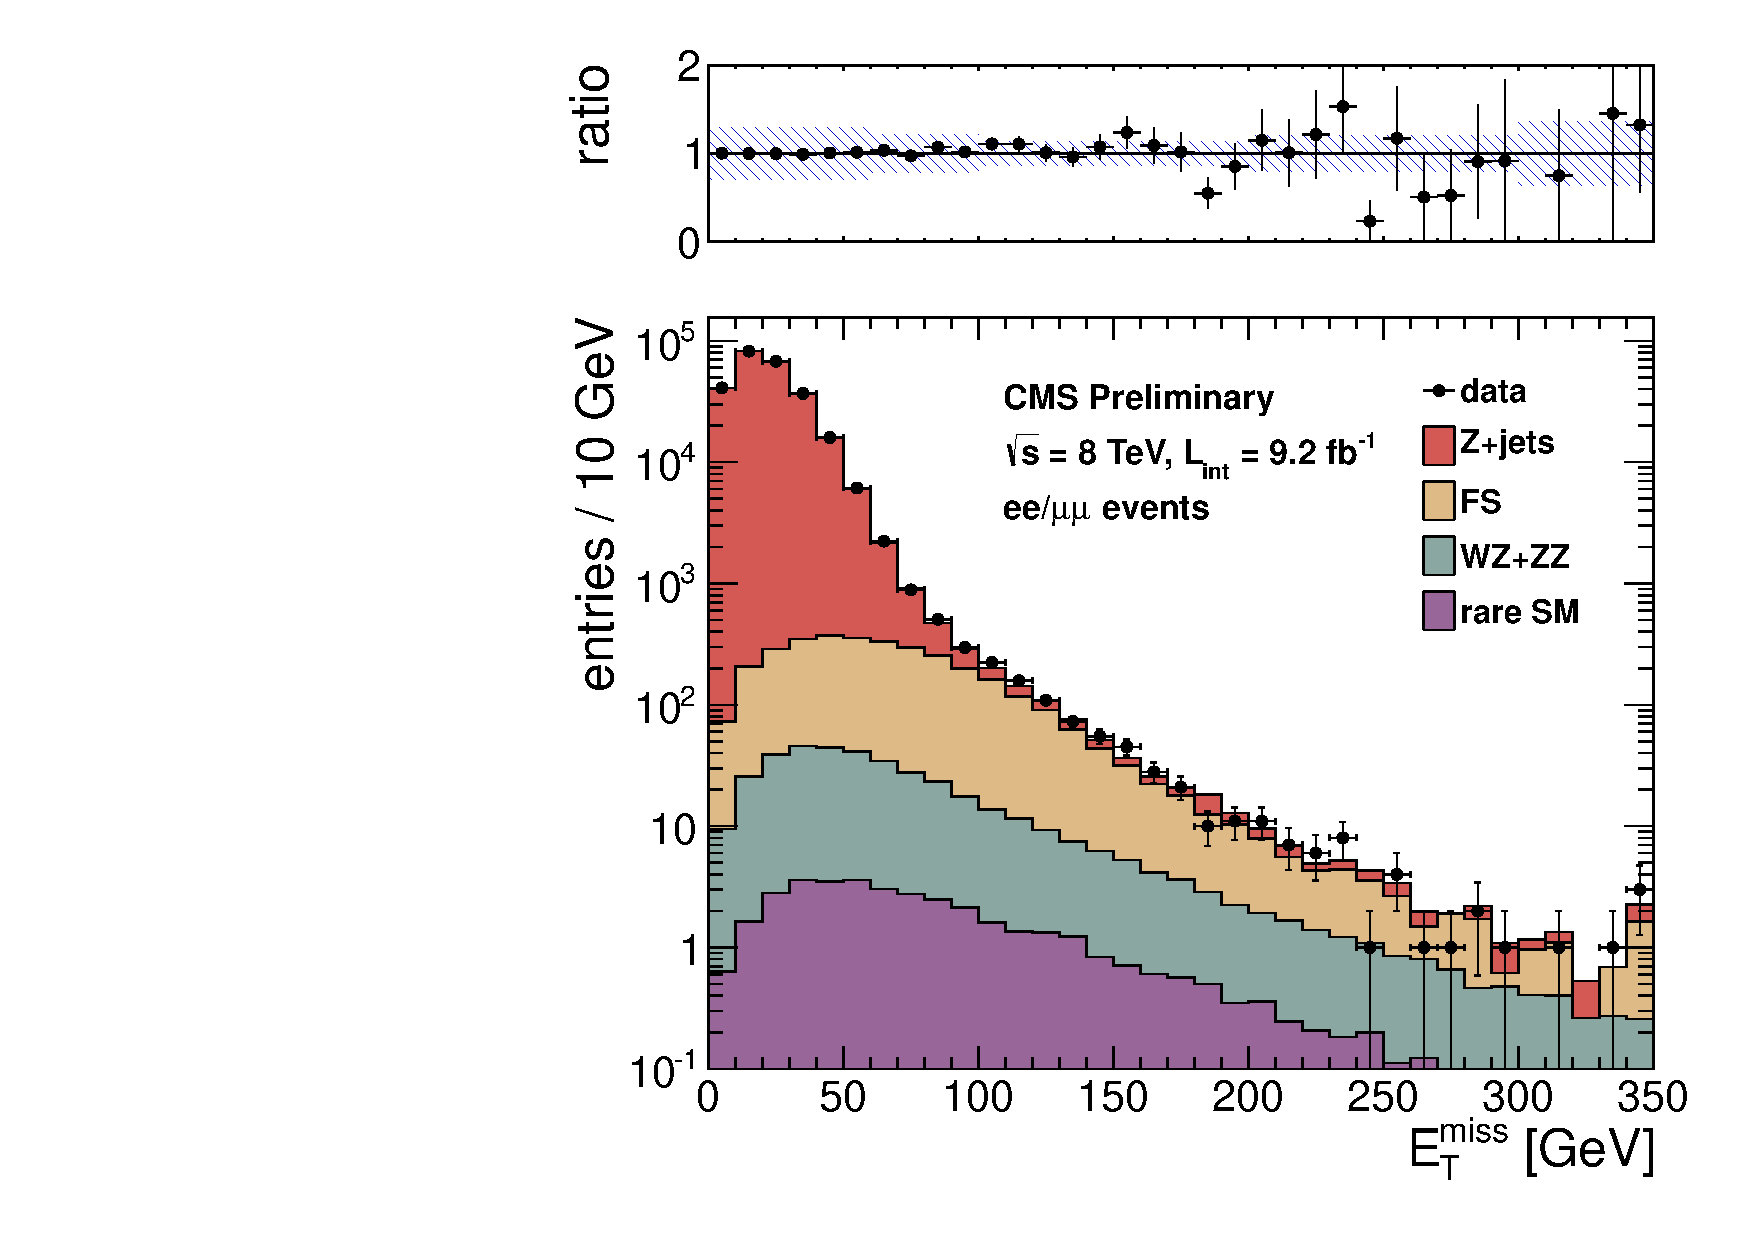
\includegraphics[width=0.6\textwidth]{plots/pfmet_all.pdf}
\end{tabular}
\caption{Results of the inclusive analysis. The observed \MET\ distribution (black points) is compared with the sum of the predicted \MET\
distributions from \zjets, flavor-symmetric backgrounds, and WZ+ZZ backgrounds. The ratio of observed to predicted yields in each bin is
indicated. The error bars indicate the statistical uncertainty in the data and the shaded band indicates the total background uncertainty.
\label{fig:results_incl}
}
\end{center}
\end{figure}



\begin{table}[htb]
\begin{center}
\footnotesize
\caption{\label{tab:results_incl} Summary of results in the inclusive analysis. The total background is the sum of the \zjets\ background predicted from
the \MET\ templates method (\zjets\ bkg), the flavor-symmetric background predicted from e$\mu$ events (FS bkg), and the WZ and ZZ backgrounds predicted from MC
(WZ bkg and ZZ bkg). All uncertainties include both the statistical and systematic components. The Gaussian significance of the deviation between the data 
and total background is indicated for signal regions with at least 20 observed events. }
\begin{tabular}{l|c|c|c|c|c|c}

\hline
\hline

\begin{comment}
Using pfmet out-of-the-box
WZ/ZZ selection : ((((((leptype==0 && (ee==1 || isdata==0))||(leptype==1 && (mm==1 || isdata==0)))&&(ngennu>0))&&(csc==0 && hbhe==1 && hcallaser==1 && ecaltp==1 && trkfail==1 && eebadsc==1 && hbhenew==1))&&(dilmass>81 && dilmass<101))&&(njets>=2))&&(lep1.pt()>20.0 && lep2.pt()>20.0)
WZ/ZZ weight    : weight * 9.2 * vtxweight * trgeff
Opening ../output/V00-01-04/babylooper_data_ALL_53X_PhotonStitchedTemplate_pfmet.root
B-veto?   0
K         0.14
ee+mm channels: scale em yield by 0.99
Yields in 0-60 GeV region
data   : 249746
gjets  : 251562
OF     : 1439.5
WZ     : 166.254
ZZ     : 23.7736
Rare   : 15.776
Scaling gjets by : 0.986239
SF events 254447
OF events 21285

ee/#mu#mu events
\end{comment}
                      &   \MET\ 0--30 GeV   &  \MET\ 30--60 GeV   & \MET\ 60--100 GeV   &\MET\ 100--200 GeV   &\MET\ 200--300 GeV   & \MET\ $>$ 300 GeV  \\
\hline
        \zjets\ bkg   &190111 $\pm$ 57034   & 57989 $\pm$ 17398   &    2744 $\pm$ 824   &      123 $\pm$ 37   &     7.4 $\pm$ 2.4   &     1.3 $\pm$ 0.5  \\
             FS bkg   &      492 $\pm$ 77   &     947 $\pm$ 147   &     981 $\pm$ 152   &      503 $\pm$ 78   &    23.6 $\pm$ 7.1   &     3.0 $\pm$ 1.9  \\
             WZ bkg   &   61.5 $\pm$ 43.0   &  104.8 $\pm$ 73.4   &   75.4 $\pm$ 52.8   &   41.2 $\pm$ 28.8   &     5.6 $\pm$ 3.9   &     1.6 $\pm$ 1.6  \\
             ZZ bkg   &     7.6 $\pm$ 3.8   &    16.2 $\pm$ 8.1   &    17.4 $\pm$ 8.7   &    16.1 $\pm$ 8.1   &     3.2 $\pm$ 1.6   &     1.0 $\pm$ 1.0  \\
        rare SM bkg   &     5.1 $\pm$ 2.5   &    10.7 $\pm$ 5.4   &    10.4 $\pm$ 5.2   &     9.1 $\pm$ 4.6   &     1.7 $\pm$ 0.8   &     0.6 $\pm$ 0.6  \\
\hline
          total bkg   &190678 $\pm$ 57034   & 59068 $\pm$ 17398   &    3829 $\pm$ 840   &      692 $\pm$ 92   &    41.5 $\pm$ 8.7   &     7.5 $\pm$ 2.7  \\
               data   &            190793   &             58953   &              3921   &               733   &                42   &                 5  \\
       significance   &       0.0$\sigma$   &      -0.0$\sigma$   &       0.1$\sigma$   &       0.4$\sigma$   &       0.0$\sigma$   &                    \\
\hline
\hline
\end{tabular}
\end{center}
\end{table}

\clearpage

The observed and predicted \MET\ distributions for the targeted analysis are indicated in Fig.~\ref{fig:results_targ}. A summary of the 
results in the signal regions is provided in Table~\ref{tab:results_targ}. 
%Here the results in the signal regions with \MET $>$ 100 GeV region are also blinded, pending completion of signal optimization studies
%(see Sec.~\ref{sec:optimization}).
The observed yields are in good agreement with the predicted background the low \MET\ region, validating the background estimation
methodology. In the signal regions defined by requirements of large \MET, good agreement is found between the observed yields and
the predicted background.

\begin{figure}[!h]
\begin{center}
\begin{tabular}{cc}
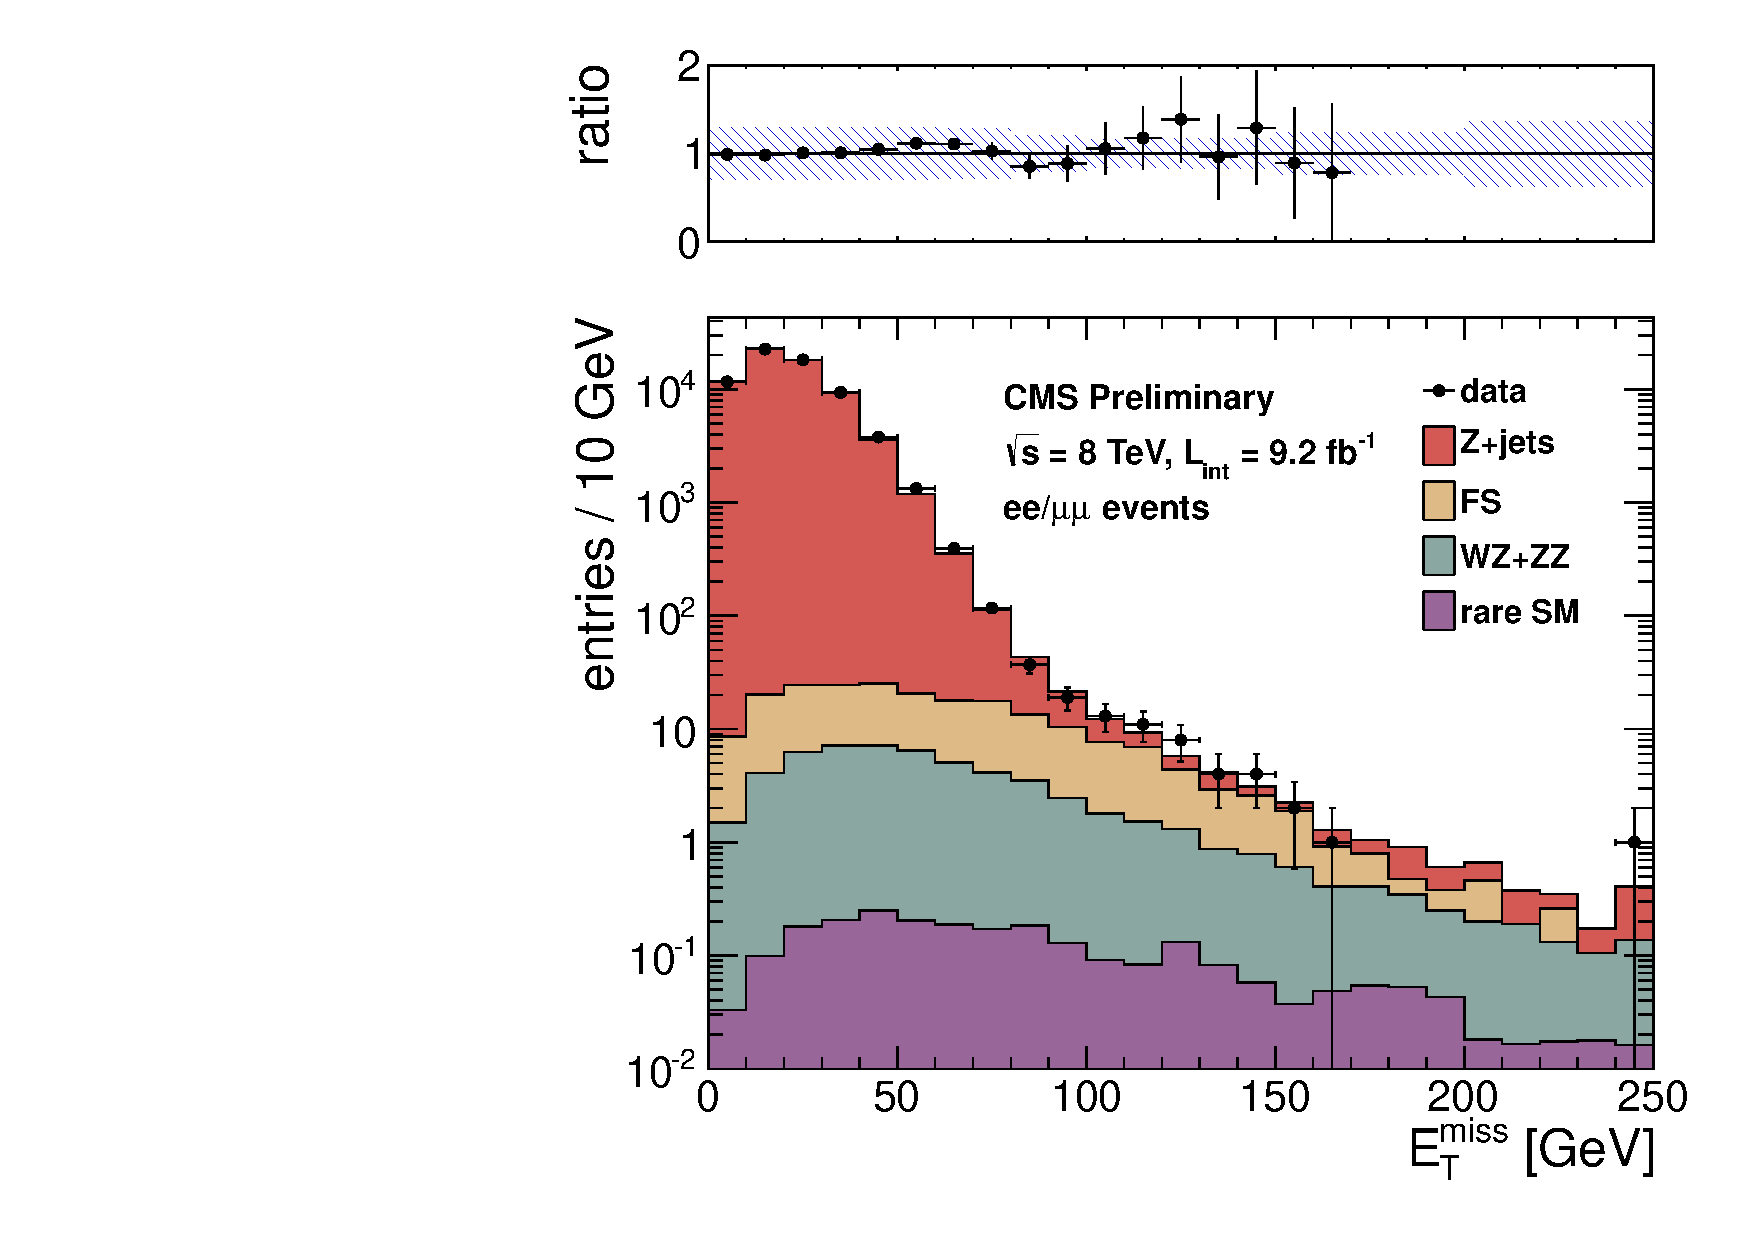
\includegraphics[width=0.5\textwidth]{plots/pfmet_bvetoMedium_all.pdf}
\end{tabular}
\caption{Results of the targeted analysis. The observed \MET\ distribution (black points) is compared with the sum of the predicted \MET\
distributions from \zjets, flavor-symmetric backgrounds, and WZ+ZZ backgrounds. The ratio of observed to predicted yields in each bin is
indicated. The error bars indicate the statistical uncertainty in the data and the shaded band indicates the total background uncertainty.
\label{fig:results_targ}
}
\end{center}
\end{figure}



\begin{table}[htb]
\begin{center}
\footnotesize
\caption{\label{tab:results_targ}\footnotesize Summary of results in the targeted analysis. The total background is the sum of the \zjets\ background predicted from
the \MET\ templates method (\zjets\ bkg), the flavor-symmetric background predicted from e$\mu$ events (FS bkg), and the WZ and ZZ backgrounds predicted from MC
(WZ bkg and ZZ bkg). All uncertainties include both the statistical and systematic components. The Gaussian significance of the deviation between the data 
and total background is indicated for signal regions with at least 20 observed events. }
\begin{tabular}{l|c|c|c|c}

\hline
\hline

                      &   \MET\ 0--30 GeV   &  \MET\ 30--60 GeV   &  \MET\ 60--80 GeV   & \MET\ 80--100 GeV   \\
\hline
        \zjets\ bkg   & 52823 $\pm$ 15847   &  14015 $\pm$ 4205   &     433 $\pm$ 130   &   40.9 $\pm$ 12.4   \\
             FS bkg   &    41.3 $\pm$ 7.2   &    49.5 $\pm$ 8.6   &    26.4 $\pm$ 4.7   &    17.9 $\pm$ 3.3   \\
             WZ bkg   &     9.5 $\pm$ 6.6   &   15.9 $\pm$ 11.2   &     6.6 $\pm$ 4.7   &     3.9 $\pm$ 2.7   \\
             ZZ bkg   &     2.1 $\pm$ 1.0   &     4.1 $\pm$ 2.1   &     2.2 $\pm$ 1.1   &     1.8 $\pm$ 0.9   \\
        rare SM bkg   &     0.3 $\pm$ 0.2   &     0.7 $\pm$ 0.3   &     0.4 $\pm$ 0.2   &     0.3 $\pm$ 0.2   \\
\hline
          total bkg   & 52876 $\pm$ 15847   &  14085 $\pm$ 4205   &     468 $\pm$ 130   &   64.7 $\pm$ 13.2   \\
               data   &             52485   &             14476   &               510   &                56   \\
       significance   &      -0.0$\sigma$   &       0.1$\sigma$   &       0.3$\sigma$   &      -0.6$\sigma$   \\


\hline
\hline

                      &\MET\ 100--120 GeV   &\MET\ 120--150 GeV   &\MET\ 150--200 GeV   & \MET\ $>$ 200 GeV  \\
\hline
        \zjets\ bkg   &     7.0 $\pm$ 2.2   &     3.1 $\pm$ 0.9   &     1.6 $\pm$ 0.5   &     0.8 $\pm$ 0.3  \\
             FS bkg   &    11.3 $\pm$ 2.2   &     6.9 $\pm$ 1.5   &     2.4 $\pm$ 1.1   &     0.4 $\pm$ 0.3  \\
             WZ bkg   &     2.1 $\pm$ 1.5   &     1.6 $\pm$ 1.1   &     1.0 $\pm$ 0.7   &     0.5 $\pm$ 0.5  \\
             ZZ bkg   &     1.0 $\pm$ 0.5   &     1.1 $\pm$ 0.6   &     0.8 $\pm$ 0.4   &     0.7 $\pm$ 0.7  \\
        rare SM bkg   &     0.2 $\pm$ 0.1   &     0.3 $\pm$ 0.1   &     0.2 $\pm$ 0.1   &     0.2 $\pm$ 0.2  \\
\hline                                                                                                         
          total bkg   &    21.7 $\pm$ 3.5   &    13.0 $\pm$ 2.2   &     6.1 $\pm$ 1.5   &     2.5 $\pm$ 0.9  \\
               data   &               ?     &             ?        &           ?          &        ?         \\
       significance   &               ?     &             ?        &           ?          &        ?         \\

\hline
\hline

\end{tabular}
\end{center}
\end{table}

\clearpage
